\subsection{\texttt{notched\_prism}}
\label{subsec:geometry_notched_prism}

\noindent
\textbf{Geometry ID:} \texttt{GLOB-GEO0004}
\qquad
\textbf{Version:} \texttt{1.0.0}

\begin{figure}[htbp]
    \centering
    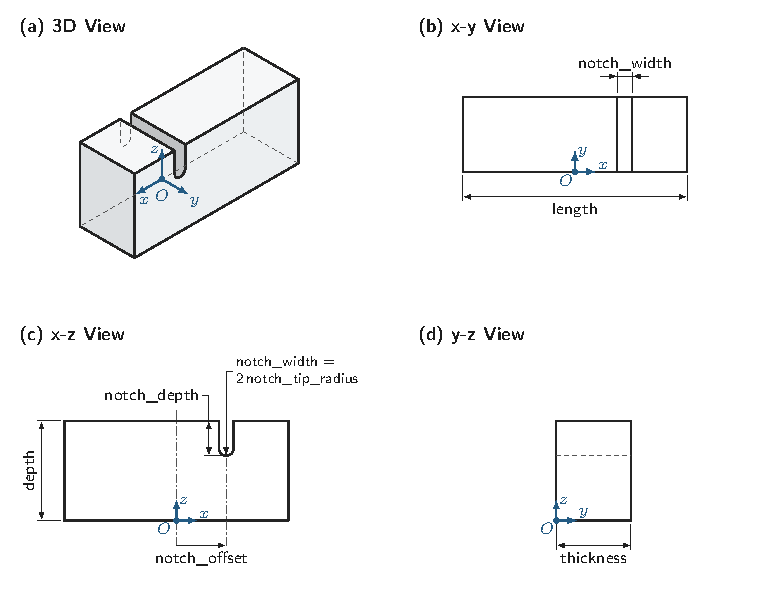
\includegraphics[width=0.65\linewidth]
    {./figs/geometries/notched_prism.pdf}
    \caption{Standardized parametrization and local
    coordinate system of the notched prism geometry.}
    \label{fig:notched_prism}
\end{figure}

The \texttt{notched\_prism} geometry represents a rectangular
prismatic specimen containing a notch with parallel sides
and a semicircular tip. As illustrated in
Fig.~\ref{fig:notched_prism}, the local coordinate system
is defined by the right-handed Cartesian axes $x$, $y$,
and $z$. The origin $O$ is located at longitudinal midspan
on the intersection of the reference face $y=0$ and
the face $z=0$.

The $x$ axis represents the longitudinal direction,
the $y$ axis the transverse thickness direction,
and the $z$ axis the specimen depth direction.
Relative to the origin, the specimen occupies the region
$-\texttt{length}/2 \leq x \leq \texttt{length}/2$,
$0 \leq y \leq \texttt{thickness}$, and
$0 \leq z \leq \texttt{depth}$.

\paragraph{Independent parameters.}

The geometry is defined by six required parameters,
all expressed in millimeters:

\begin{itemize}
    \item \texttt{length}: specimen dimension along
    the local $x$ axis;

    \item \texttt{thickness}: specimen dimension along
    the local $y$ axis;

    \item \texttt{depth}: specimen dimension along
    the local $z$ axis;

    \item \texttt{notch\_offset}: signed $x$ coordinate
    of the notch centerline relative to specimen
    midspan. A value of zero corresponds to a
    centered notch;

    \item \texttt{notch\_depth}: positive distance
    from the notched face to the deepest point
    of the semicircular notch tip, measured
    along the local $z$ direction;

    \item \texttt{notch\_width}: opening width
    of the notch.
\end{itemize}

\paragraph{Derived parameters.}

The notch terminates in a semicircular tip whose
radius is determined by the notch opening width:

\begin{equation}
    \texttt{notch\_tip\_radius}
    = \frac{\texttt{notch\_width}}{2}.
\end{equation}

Consequently, \texttt{notch\_tip\_radius} is a
derived quantity and is not an independent input
parameter.

\paragraph{Geometric constraints.}

All dimensions must be strictly positive, with
the exception of \texttt{notch\_offset}, which
may be positive, negative, or zero.

The notch geometry must additionally satisfy

\begin{align}
    \texttt{notch\_depth}
    &> \frac{\texttt{notch\_width}}{2},
    \\
    \texttt{notch\_depth}
    &< \texttt{depth},
    \\
    \texttt{notch\_offset}
    + \frac{\texttt{notch\_width}}{2}
    &< \frac{\texttt{length}}{2},
    \\
    \frac{\texttt{notch\_width}}{2}
    - \texttt{notch\_offset}
    &< \frac{\texttt{length}}{2}.
\end{align}

The first condition ensures that the notch contains
a straight-sided segment preceding its semicircular
termination. The second prevents the notch from
penetrating the full specimen depth, while the
remaining conditions ensure that the notch remains
within the longitudinal boundaries of the specimen.
